\begin{pastexam}[label={px:ntut-112-ee-ds-08}]{北科大電機所（戊組）112 學年度 第 8 題}
（追蹤）

Consider the tree below, show the output for each of functions:
\begin{center}
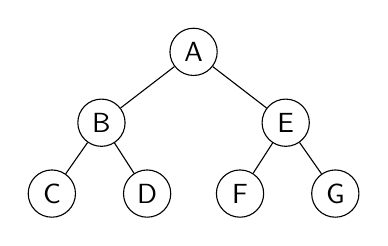
\begin{tikzpicture}[v/.style={circle,draw,inner sep=1pt,minimum size=6mm,font=\sffamily}]
\node[v] (nA) at (2.07,0.00) {A};
\node[v] (nB) at (0.90,-0.90) {B};
\node[v] (nE) at (3.24,-0.90) {E};
\node[v] (nC) at (0.27,-1.80) {C};
\node[v] (nD) at (1.48,-1.80) {D};
\node[v] (nF) at (2.66,-1.80) {F};
\node[v] (nG) at (3.87,-1.80) {G};
\draw (nA) -- (nB);
\draw (nA) -- (nE);
\draw (nB) -- (nC);
\draw (nB) -- (nD);
\draw (nE) -- (nF);
\draw (nE) -- (nG);
\end{tikzpicture}
\end{center}
\noindent\begin{tabular}{|p{0.45\linewidth}|p{0.45\linewidth}|}
\hline
(a)Given the following:
\begin{minted}[fontsize=\small]{c}
void t1(TreeNode x)
 {   if (x!=null)
   {   printf("%c",x->key);
      t1(x->right);
       t1(x->left);
       printf("%c",x->key);
   }
 }
\end{minted}
\hfill (5\%)
&
(b)Given the following:
\begin{minted}[fontsize=\small]{c}
void t2(TreeNode x)
 {   if (x!=null)
   {   t1(x->left);
       t1(x->right);
       printf("%c",x->key);
       t1(x->left);
   }
 }
\end{minted}
\hfill (5\%)
\\ \hline
\end{tabular}
\end{pastexam}

\begin{pastsoln}
樹：A 的左、右子節點是 B、E；B 的是 C、D；E 的是 F、G。

\textbf{(a)} 答案：\texttt{AEGGFFEBDDCCBA}。

\texttt{t1(x)} 先印 $x$、再走\textbf{右}子樹、再走\textbf{左}子樹、最後再印一次 $x$。 每個節點印兩次，一次在進入時、一次在
離開時（像括號），而且先右後左。 葉節點 $y$ 的 \texttt{t1(y)} 印出 $yy$。
\begin{itemize}
\item \texttt{t1(E)} $=$ E $+$ \texttt{t1(G)} $+$ \texttt{t1(F)} $+$ E $=$ E GG FF E。
\item \texttt{t1(B)} $=$ B $+$ \texttt{t1(D)} $+$ \texttt{t1(C)} $+$ B $=$ B DD CC B。
\item \texttt{t1(A)} $=$ A $+$ \texttt{t1(E)} $+$ \texttt{t1(B)} $+$ A $=$ A EGGFFE BDDCCB A。
\end{itemize}
共 $14$ 個字元（$7$ 個節點各兩次）。

\textbf{(b)} 答案：\texttt{BDDCCBEGGFFEABDDCCB}。

注意 \texttt{t2} 只在最外層呼叫一次，裡面呼叫的都是 \texttt{t1}，不是 \texttt{t2}。 \texttt{t2(A)} 依序做：
\begin{enumerate}
\item \texttt{t1(B)}：BDDCCB（同 (a)）。
\item \texttt{t1(E)}：EGGFFE。
\item 印 A。
\item \texttt{t1(B)}：再一次 BDDCCB。
\end{enumerate}
接起來是 BDDCCB EGGFFE A BDDCCB，共 $6 + 6 + 1 + 6 = 19$ 個字元。
\end{pastsoln}
